
In this chapter we will analyze related data integration and dataspace works in the healthcare sector. This will help us to properly design and implement our own system.

We will cover the following works:

\begin{itemize}
\item DebugIT which has a mediator-based architecture and uses ontology-based data integration.
\item 'Dataspace Integration in the medical research' the doctor thesis of Sebastian H.R. Wurst
\end{itemize}

\section{DebugIT}
The DebugIT project is a good reference for analyzing how medical data integration can be done though this project didn't use a dataspace approach but an ontology-mediated \cite{WurstDiss, DBLP:books/dp/LeserN2006} approach. DebugIT stands for ``Detecting and Eleminating Bacteria Using Information Technology'' and its main goal is to provide a platform for high-throughput analysis of distributed clinical data as a response to the spread of antibiotic resistance of infectious pathogens in European hospitals\cite{UniFreiburgDebugITInfo}. 
The team of the DebugIT project released the architecture of their system in \cite{DBLP:conf/swat4ls/SchoberCDEDJTPLB14}.
In that paper it is stated, that the system uses an ontology-based approach for allowing antibiotics resistance data being semantically and geographically interoperable. This makes it possible to integrate distributed clinical data EU-wide in real-time for monitoring antibiotic resistance. As well, the system is structured in four tiers and works in a service oriented manner (SOA). Figure \ref{DebugITArchitectureFigure} shows the layered architecture of the system of DebugIT.

\begin{figure}[]
	\begin{center}
		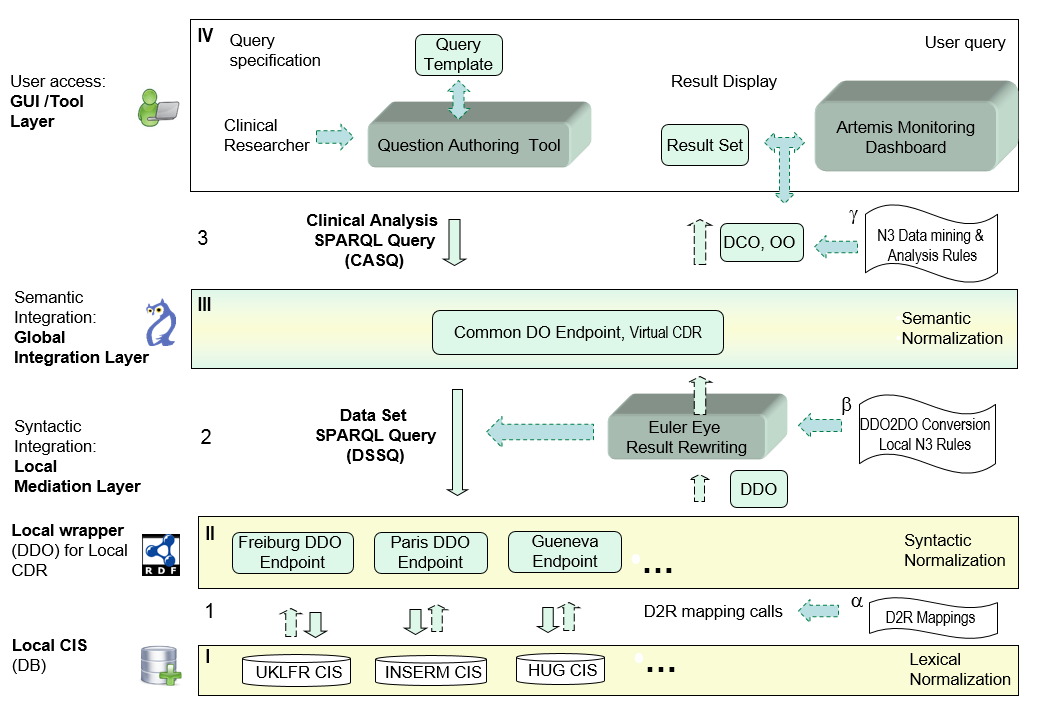
\includegraphics[width=0.75\textwidth]{figures/DebugIT-Ontology-mediated-layered-Data-Integration-architecture.png}
	\end{center}
	\caption{The layered mediator architecture of the DebugIT project}
	\label{DebugITArchitectureFigure}
\end{figure}

Altogether there are 3 data representation layers marked with the Roman Numerals I-III. The query flow between the data layers is specified with 1-3 and the corresponding mappings are given with the Greek letters \textalpha , \textbeta,  and \textgamma .

On the first integration layer (\textbf{I}) relational data are lexical normalized by the use of mappings of medical terminology and morphosemantic mapping employed by the Averbis Morphosaurus software\cite{DaumkeDiss}. Ambiguities can be resolved with ontological expressions (formulated in OWL) on the integration layers II and III. 

The layer \textbf{II} works with RDF data, wherefore relational data from the layer I is transformed to RDF through D2R mapping calls \footnote{http://d2rq.org/} on the\emph{ first mediation layer} (1). On the second integration layer information about the data and their corresponding vocabulary is stored in Data Definition Ontologies (DDOs) \cite{DebugITDDO}. A DDO bridges a local data model and a semi-formal data model on the local mediation layer for integrating syntactic data and provides an Extract, Transform, Load (ETL)-process \footnote{DBLP:books/dp/LeserN2006} for the next integration layer. So materialized data integration is partially done on this layer.
For each Clinical Data Repository (CDR) such a DDO is locally created. A CDR contains clinical data of a specific hospital, institute or is a compound of CDRs.
Layer II contains also a SPARQL endpoint, for allowing Layer III to query its data. These queries are specified through a Data Set SPARQL Query (DSSQ). 

On the \emph{second mediation layer} (2), in the figure called local mediation layer, the local DDO data is bind to the global DebugIT Core Ontology (DCO) \cite{Schober_developingdco:}, which s the ontology of layer III. The corresponding mapping is done through DDO2DCO using the N3 language \footnote{http://www.w3.org/TeamSubmission/n3/} and Simple Knowledge Organization Structure (SKOS) mappings \footnote{http://www.w3.org/TR/2009/REC-skos-reference-20090818/}. The schema mapping is done by the Euler Eye Reasoner \footnote{http://eulersharp.sourceforge.net/}, which also creates implicit knowledge using logical inference.

Data layer \textbf{III} represents a virtual Clinical Data Repository (vCDR), which joins the local Clinical Information Systems (CISs). Important to know is, that in the vCDR are now fully (semantically) integrated and as the name implies, a vCDR \emph{virtually} integrates the data. So data is not duplicated anymore. Through the virtualisation, data of all CIS can be globally queried. Also privacy issues can properly be handled, as the data is not stored outside from the CISs.
Also on layer III clinical analyses can be performed over Clinical Analysis SPARQL Queries (CASQ (3)). 

On the last layer (\textbf{IV}), a user or a monitoring tool can query the integrated clinical data.

Summarizing it, the mapping is performed iteratively in a stack-like manner:
The first mapping \textalpha (D2R mappings) transforms the relational database layer (I) to the RDF representation layer (II). The next mapping \textbeta (N3 and SKOS) transforms the RDF layer II to the Domain Ontology (OO) layer III, where the data is globally queryable as CASQ over mapping \textgamma (DCO and OO).  

\section{Dataspace Integration in the medical research}

'Dataspace Integration in the medical research' (original title 'Dataspace Integration in der medizinischen Forschung') is a german doctor thesis, was written by Sebastian H.R. Wurst and submitted in 2010 \cite{WurstDiss}.

\begin{figure}[H]
	\begin{center}
		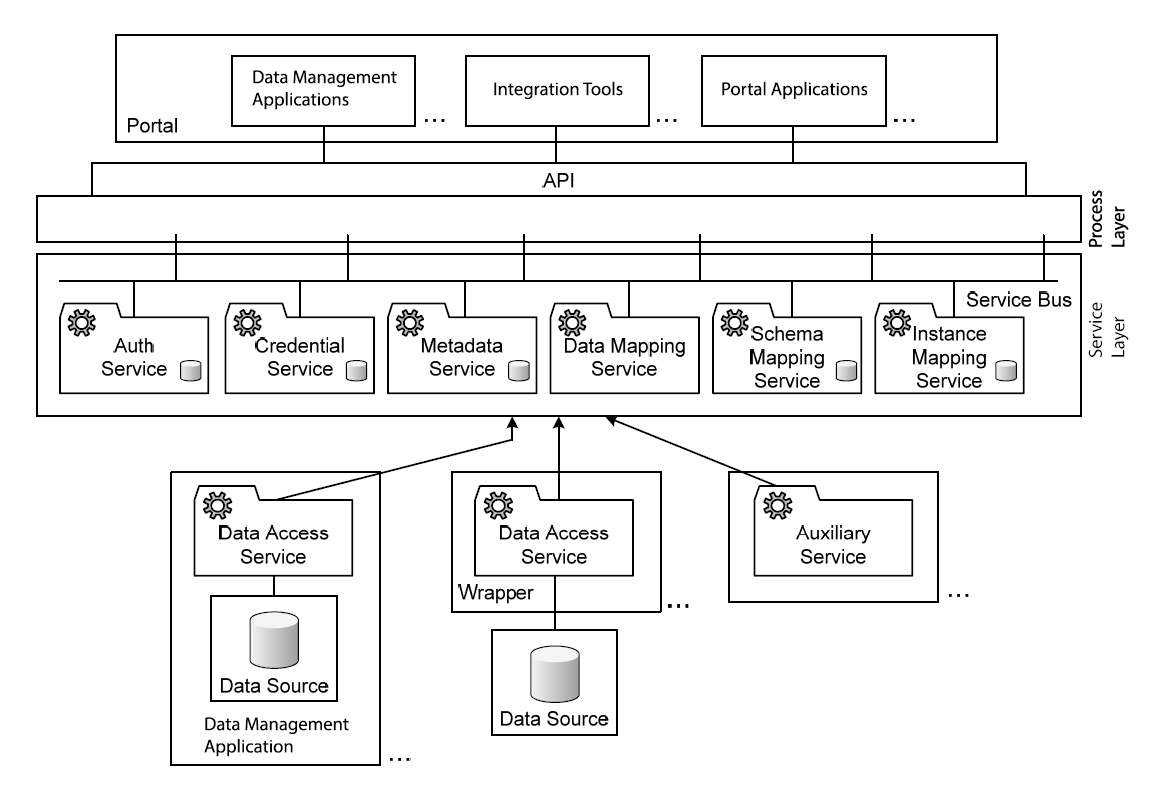
\includegraphics[width=0.9\textwidth]{figures/DataspaceIntegrationInDerMedForschungFigure31.PNG}
	\end{center}
	\caption{Overview of the software architecture of the system used in the doctor thesis of Sebastian H.R. Wurst \cite[p. 117, Figure 31]{WurstDiss}}
	\label{DebugITArchitectureFigure}
\end{figure}